\documentclass{beamer}

\usepackage[lined,ruled]{algorithm2e}
\usepackage{subfigure}
\usepackage[english]{babel}
\usepackage[latin1]{inputenc}
\usepackage{times}
\usepackage[T1]{fontenc} 
\usepackage{color}

\usetheme[secheader]{Boadilla}
\usefonttheme[onlylarge]{structurebold}
\setbeamerfont*{frametitle}{size=\normalsize,series=\bfseries}
\setbeamertemplate{navigation symbols}{}
\setbeamertemplate{mini frames}[box]
\setbeamertemplate{sections/subsections in toc}[square]
\setbeamertemplate{blocks}[rounded][shadow=true]
\setbeamertemplate{bibliography item}[text]

\setbeamercolor{lightorange}{fg=black,bg=orange!40}
\setbeamercolor{lightblue}{fg=black,bg=blue!30}

\newenvironment{colorblock}[2]
{\setbeamercolor{item}{fg=#1,bg=#1}\begin{beamerboxesrounded}[upper=#1,lower=#2,shadow=true]}
  {\end{beamerboxesrounded}}



% Setup TikZ

\usepackage{tikz}
\usetikzlibrary{arrows}
\tikzstyle{block}=[draw opacity=0.7,line width=1.4cm]


%%%%%%%%%%%%%%%%%%%%%%%%%%%%%%%%%%%%%
%%%%%%%%%%%%%%%%%%%%%%%%%%%%%%%%%%%%%
%%%%%%%%%%%%%%%%%%%%%%%%%%%%%%%%%%%%%

\newtheorem{observation}[theorem]{Observation} 

%%%%%%%%%%%%%%%%%%%%%%%%%%%%%%%%%%%%%
%%%%%%%%%%%%%%%%%%%%%%%%%%%%%%%%%%%%%
%%%%%%%%%%%%%%%%%%%%%%%%%%%%%%%%%%%%%

\title{Coordinating Distributed Systems}
\subtitle{Theory and practice}
\author{Daniele Venzano}
\institute{Eurecom}
\date


\begin{document}

\begin{frame}
  \titlepage
\end{frame}

%%%%%%%%%%%%%%%%%%%%%%%%%%%%%%%%%%%%%%%%%%%%%%%%%%%%%%%%%%
%%%%%%%%%%%%%%%%%%%%%%%%%%%%%%%%%%%%%%%%%%%%%%%%%%%%%%%%%%
\section{Introduction}

\begin{frame}
 \begin{colorblock}{blue}{lightblue}{ }
  \begin{center}
    \Huge \textbf{\texttt{Introduction}}
  \end{center}
  \end{colorblock}
\end{frame}

%%%%%%%%%%%%%%%%%%%%%%%%%%%%%%%%%%%%%%%%%%%%%%%%%%%%%%%%%%
\frame {\frametitle{Outline}
	\begin{itemize}
		\item \textbf{What is a distributed system?}
		
		\vspace{7pt}
		
		\item \textbf{The consensus problem}
		\begin{itemize}
			\item A few examples of distributed consensus
			\item CAP theorem
			\item Eventually consistent Vs Strongly consistent
			\item Fault tolerance: possible faults in distributed systems
		\end{itemize}
		
		\vspace{7pt}
		
		\item \textbf{Consensus protocols}
		\begin{itemize}
			\item Raft from A to Z
			\item Paxos overview
			\item Other protocols
		\end{itemize}
		
		\vspace{7pt}
		
		\item \textbf{Implementations - ZooKeeper}
		\begin{itemize}
			\item History
			\item Architecture
			\item Data model
			\item Higher-level primitives
		\end{itemize}
			
	\end{itemize}
}
%%%%%%%%%%%%%%%%%%%%%%%%%%%%%%%%%%%%%%%%%%%%%%%%%%%%%%%%%%
\subsection{What is a distributed system?}
\frame {\frametitle{What is a distributed system?}
	\begin{center}
		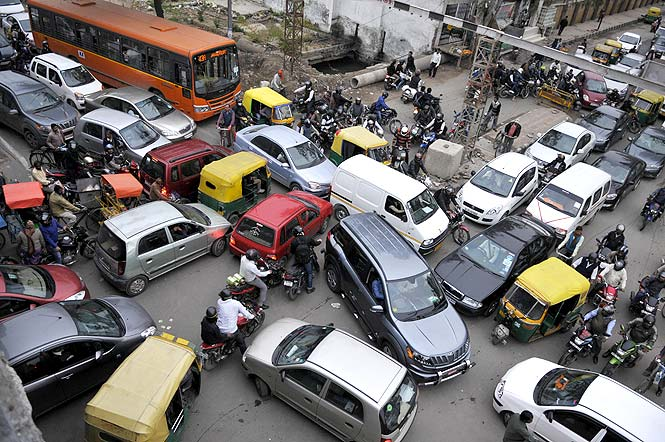
\includegraphics[width=0.6\textwidth]{images/traffic-jam}
	\end{center}
	\begin{itemize}
		\item A set of processes seeking to achieve some common goal by communicating with each other
	\end{itemize}
}

%%%%%%%%%%%%%%%%%%%%%%%%%%%%%%%%%%%%%%%%%%%%%%%%%%%%%%%%%%
\frame {\frametitle{What is a distributed system?}
	\begin{itemize}
		\item Like a software matrioshka
		\begin{itemize}
			\item Multi-threaded process
			\item Multi-process on a single server
			\item \textbf{Multiple processes in a set of servers in the same datacenter}
			\item \textbf{Multiple processes in a set of geographically distributed servers}
		\end{itemize}
	
		\vspace{10pt}
	
		\item Why?
		\begin{itemize}
			\item Inherent distribution (sensors, peer-to-peer, publish-subscribe, ...)
			\item Engineering choice (fault tolerance, replication, performance, ...)
		\end{itemize}
	
		\vspace{10pt}
		
		\item These processes need to coordinate to reach a common goal:
		\begin{itemize}
			\item data aggregation
			\item synchronization
			\item transactions
			\item ...
		\end{itemize}
	\end{itemize}
}

%%%%%%%%%%%%%%%%%%%%%%%%%%%%%%%%%%%%%%%%%%%%%%%%%%%%%%%%%%
%%%%%%%%%%%%%%%%%%%%%%%%%%%%%%%%%%%%%%%%%%%%%%%%%%%%%%%%%%

\section{The consensus problem}
\begin{frame}
 \begin{colorblock}{blue}{lightblue}{ }
  \begin{center}
    \Huge \textbf{\texttt{The consensus problem}}
  \end{center}
  \end{colorblock}
\end{frame}

%%%%%%%%%%%%%%%%%%%%%%%%%%%%%%%%%%%%%%%%%%%%%%%%%%%%%%%%%%
\subsection{Examples of the consensus problem}
\frame {\frametitle{Wedding consensus}
	\begin{itemize}
		\item The priest follows a well known protocol to reach a consensus:
		\begin{enumerate}
			\item Priest: Alice, will you marry Bob ?
			\item Alice: yes
			\item Priest: Bob, will you marry Alice ?
			\item Bob: yes
			\item Priest: You are now husband and wife
		\end{enumerate}

		\vspace{10pt}

		\item In distributed systems this becomes:
		\begin{enumerate}
			\item Coordinator: Alice, can you commit key X with value 5 ?
			\item Alice: yes, I can
			\item Coordinator: Bob, can you commit key X with value 5 ?
			\item Bob: yes, I can
			\item Coordinator: Ok, both of you record that X has now a value of 5
		\end{enumerate}

		\vspace{10pt}

		\item What if Bob flees from the church?
	\end{itemize}
}
%%%%%%%%%%%%%%%%%%%%%%%%%%%%%%%%%%%%%%%%%%%%%%%%%%%%%%%%%%
\frame {\frametitle{The two generals}
	\begin{center}
		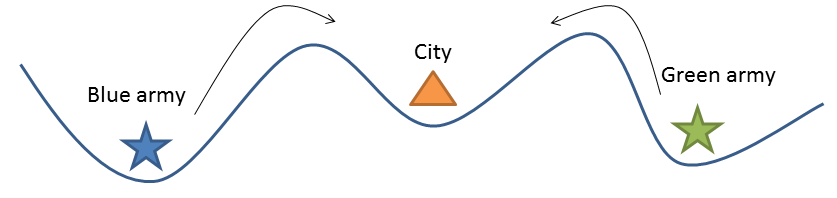
\includegraphics[width=\textwidth]{images/2generals}
	\end{center}
	\begin{itemize}
	\item Two generals want to attack a city
	\item They can only use unreliable messengers to communicate
	\item They need to attack at the same time to succeed
	\end{itemize}

	An infinite number of messages is needed for each general to be sure the other agrees on the time of the attack.
}

%%%%%%%%%%%%%%%%%%%%%%%%%%%%%%%%%%%%%%%%%%%%%%%%%%%%%%%%%%
\frame {\frametitle{Consensus examples}
	Processes need to reach a common goal:
	\begin{itemize}
		\item aggregate functions: sensors calculating average temperature
		\item synchronization: agree on a value, elect a leader
		\item reliable broadcast: a message sent to a group is received by all or none
		\item atomic commit: ensure that processes reach a common decision whether to commit or abort a transaction
	\end{itemize}
}

%%%%%%%%%%%%%%%%%%%%%%%%%%%%%%%%%%%%%%%%%%%%%%%%%%%%%%%%%%
\frame {\frametitle{Properties of a distributed system}
	\begin{itemize}
		\item Linearizability\footnote{The CAP theorem calls Consistency what is actually Linearizability}: a given set of operations is \emph{linearizable} if it appears to the rest of the system to occur instantaneously
		\begin{itemize}
			\item Writes are linearizable operations if every read receives the most recent write or an error
		\end{itemize}
		\item Availability: a system is \emph{available} if every request to a non-failing node always receives a response, eventually
		\begin{itemize}
			\item Reading stale data is ok, though
		\end{itemize}
		\item Partition tolerance
		\begin{itemize}
			\item The system continues to function properly even if the network loses or delays an arbitrary number of messages
		\end{itemize}
	\end{itemize}

	The CAP theorem links these three properties.
}

%%%%%%%%%%%%%%%%%%%%%%%%%%%%%%%%%%%%%%%%%%%%%%%%%%%%%%%%%%
\frame {\frametitle{CAP theorem - 1}
	The theorem says: between C A P, you can choose only two
	\begin{center}
		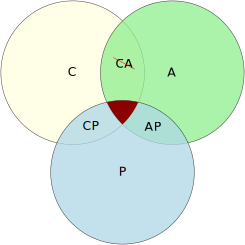
\includegraphics[width=0.5\textwidth]{images/cap}
	\end{center}
	(... but you need the P ...)
}

%%%%%%%%%%%%%%%%%%%%%%%%%%%%%%%%%%%%%%%%%%%%%%%%%%%%%%%%%%
\frame {\frametitle{CAP theorem - 2 - Why not all three?}
	\begin{center}
		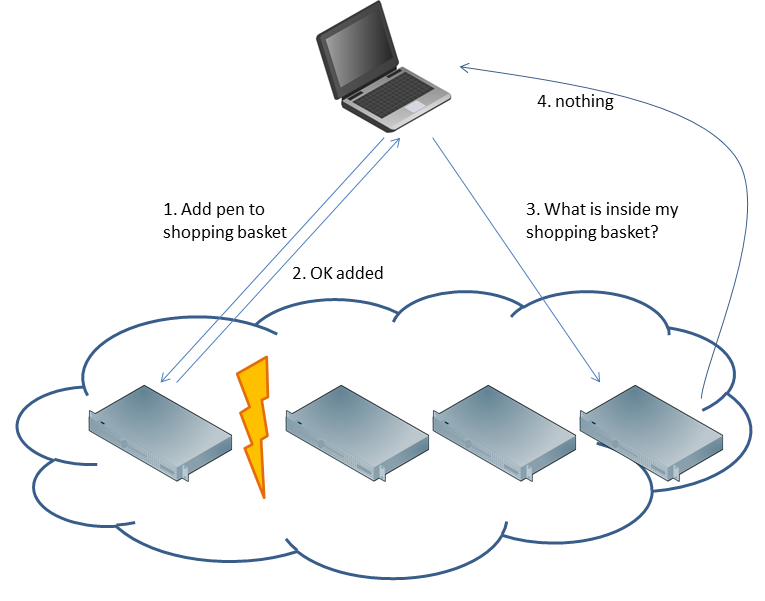
\includegraphics[width=0.7\textwidth]{images/cap2}
	\end{center}

	If there is a network partition either C or A will break
}

%%%%%%%%%%%%%%%%%%%%%%%%%%%%%%%%%%%%%%%%%%%%%%%%%%%%%%%%%%
\frame {\frametitle{CAP theorem - 3 - P}
	\begin{itemize}
		\item Network partitions occur outside anyone's control in real life
		\item Cannot sacrifice the Partition-Tolerance property
		\item In the event of a network partition either A or C is maintained: it is the choice of the designer
		\item Practical distributed systems are CP or AP
		\item Some can be configured to shift between CP and AP (tunable consistency)
	\end{itemize}
	
	\vspace{10pt}
	
	Note: a network partition can also be a very slow link
}

%%%%%%%%%%%%%%%%%%%%%%%%%%%%%%%%%%%%%%%%%%%%%%%%%%%%%%%%%%
\frame {\frametitle{CAP theorem - 4 - Summary}
	\begin{itemize}
		\item First stated by Eric Brewer (Berkeley) at the PODC 2000 keynote
		\item Formally proved by Gilbert and Lynch, 2002\cite{Gilbert02}
	\end{itemize}
	
	\vspace{5pt}
%	
%	\begin{enumerate}
%		\item Theorem 1: it is impossible in the \emph{asynchronous} network model to implement a read/write variable that guarantees availability (A) and consistency (C) in all executions (including those in which messages are lost)
%		\item Theorem 2: the same applies to the \emph{partially synchronous} network model
%	\end{enumerate}

%	\vspace{5pt}
	
%	\begin{itemize}
%		\item asynchronous: no clocks, message delays unbounded
%		\item partially synchronous: bounds on the time it takes to deliver and process messages, but clocks are not synchronized and messages can be lost
%	\end{itemize}
%}

%%%%%%%%%%%%%%%%%%%%%%%%%%%%%%%%%%%%%%%%%%%%%%%%%%%%%%%%%%
%\frame {\frametitle{CAP theorem - 6 - Summary}
	\begin{itemize}
		\item The CAP theorem formally states the trade-offs among different distributed systems properties
		\item In practice network Partitions occur, the designer can choose one of Consistency or Availability
		\item The choice heavily depends on what your application/business logic is
	\end{itemize}
}

%%%%%%%%%%%%%%%%%%%%%%%%%%%%%%%%%%%%%%%%%%%%%%%%%%%%%%%%%%
\frame {\frametitle{CAP theorem - 5 - Summary}

	CP-oriented systems:
	\begin{itemize}
		\item BigTable, Hbase, MongoDB, Redis, MemCacheDB, Scalaris, Paxos, ZooKeeper$^1$
	\end{itemize}
	
	\vspace{5pt}
	
	AP-oriented systems:
	\begin{itemize}
		\item Amazon Dynamo, CouchDB, Cassandra\footnote{CA or CP tunable}, SimpleDB, Riak, Voldemort
	\end{itemize}

	In-depth articles on the misuse of the CAP theorem in describing real systems:
	\begin{itemize}
	\item \url{https://codahale.com/you-cant-sacrifice-partition-tolerance/}
	\item \url{https://martin.kleppmann.com/2015/05/11/please-stop-calling-databases-cp-or-ap.html}
	\end{itemize}
}

%%%%%%%%%%%%%%%%%%%%%%%%%%%%%%%%%%%%%%%%%%%%%%%%%%%%%%%%%%
\frame {\frametitle{Consistency models}

	\begin{itemize}
		\item Eventual consistency: after a write, every read from the distributed system will \emph{eventually} return the written value, if no new updates are made to it
	
		\vspace{5pt}
	
		\item Strong consistency: after a write, all reads from the distributed system will return either the old or the new value
	\end{itemize}
}

%%%%%%%%%%%%%%%%%%%%%%%%%%%%%%%%%%%%%%%%%%%%%%%%%%%%%%%%%%
\frame {\frametitle{Fault tolerance in distributed systems}
	Faults examples:
	\begin{itemize}
		\item Simple: network partitions, hardware or software crashes, outdated/malicious nodes (bizantine faults)
		\item Complex: feedback loops that overcompensate in good faith (examples in next slides)
	\end{itemize}

	Faults will always happen, design tolerance mechanisms:
	\begin{itemize}
		\item Replication: master-slave ($\rightarrow$ failover) or load balancing
		\item Isolation: malfunctioning components do not affect the system as a whole
	\end{itemize}
}

%%%%%%%%%%%%%%%%%%%%%%%%%%%%%%%%%%%%%%%%%%%%%%%%%%%%%%%%%%
\frame {\frametitle{Amazon DynamoDB crash (2015/09/20)}
	DynamoDB: distributed NoSQL database from Amazon web services (AWS)
	\begin{enumerate}
		\item Network disruption caused timeouts of some storage servers
		\item The affected servers tried to re-establish their membership
		\item A change of usage pattern caused membership data to be unexpectedly large
		\item Membership servers started to overload
		\item More storage servers timed-out on health checks to membership servers
		\item Cascading failure, stabilized at 55\% error rate for customers
	\end{enumerate}
	Post-mortem: \url{https://aws.amazon.com/message/5467D2/}
}

%%%%%%%%%%%%%%%%%%%%%%%%%%%%%%%%%%%%%%%%%%%%%%%%%%%%%%%%%%
\frame {\frametitle{More real-world failures}
	\begin{itemize}
		\item Google: \url{https://status.cloud.google.com/summary}
		\item Facebook: \url{https://www.facebook.com/notes/facebook-engineering/more-details-on-todays-outage/431441338919}
		\item Apple: \url{http://appleinsider.com/articles/16/06/02/apples-app-stores-apple-tv-itunes-other-services-hit-with-downtime}
		\item Microsoft (Azure): \url{https://azure.microsoft.com/en-us/status/history/}
	\end{itemize}
}

%%%%%%%%%%%%%%%%%%%%%%%%%%%%%%%%%%%%%%%%%%%%%%%%%%%%%%%%%%
%%%%%%%%%%%%%%%%%%%%%%%%%%%%%%%%%%%%%%%%%%%%%%%%%%%%%%%%%%

\section{Consensus protocols}

\begin{frame}
 \begin{colorblock}{blue}{lightblue}{ }
  \begin{center}
    \Huge \textbf{\texttt{Consensus protocols}}
  \end{center}
  \end{colorblock}
\end{frame}


\subsection{Paxos}
\subsection{Raft}
%%%%%%%%%%%%%%%%%%%%%%%%%%%%%%%%%%%%%%%%%%%%%%%%%%%%%%%%%%
%%%%%%%%%%%%%%%%%%%%%%%%%%%%%%%%%%%%%%%%%%%%%%%%%%%%%%%%%%

\section{Zookeper}

\begin{frame}
 \begin{colorblock}{blue}{lightblue}{ }
  \begin{center}
    \Huge \textbf{\texttt{ZooKeeper}}
  \end{center}
  \end{colorblock}
\end{frame}
%%%%%%%%%%%%%%%%%%%%%%%%%%%%%%%%%%%%%%%%%%%%%%%%%%%%%%%%%%
\subsection{History}
\frame {\frametitle{History}
}
%%%%%%%%%%%%%%%%%%%%%%%%%%%%%%%%%%%%%%%%%%%%%%%%%%%%%%%%%%
\subsection{Architecture}
\frame {\frametitle{Architecture}
}
%%%%%%%%%%%%%%%%%%%%%%%%%%%%%%%%%%%%%%%%%%%%%%%%%%%%%%%%%%
\subsection{Higher-level primitives}
\frame {\frametitle{Higher-level primitives}
}

%%%%%%%%%%%%%%%%%%%%%%%%%%%%%%%%%%%%%%%%%%%%%%%%%%%%%%%%%%
%%%%%%%%%%%%%%%%%%%%%%%%%%%%%%%%%%%%%%%%%%%%%%%%%%%%%%%%%%

\section{References}
\begin{frame}[allowframebreaks]{References}
\bibliographystyle{plain} 
\bibliography{references} 
\end{frame}

\end{document}
